\chapter{Ionomics and Lipidomics of the Andosol Introgression Resource Panel: Kernel Nutrient Accumulation and Potential Adaptations to Highland and Lowland Phosphorus Deficiencies}
\label{chap-three}

\newrefsection

\section{Background}
Andosols are soils of volcanic origin that support maize crops, pasture grasses, and native forests in the highlands of Mexico \citep{bayuelo-jimenez2020,galvan-tejada2014}
Although nutrient deficiency and acidity in these soils can be remedied by adding mineral or organic fertilizers \citep{nobile2020}, maize has been cultivated in the Mexican Highlands for the last 6500 years \citep{piperno2001} without industrial fertilizers.
Adaptation to low phosphorus availability is evidenced by local corn varieties that, under phosphorus deficiency, have increased phosphorus use and acquisition efficiency when grown in the Andosols of the highland plateau of the Transmexican Volcanic Belt (TMVB) \citep{bayuelo-jimenez2011,bayuelo-jimenez2014}

In this work, we use ionomics to search for quantitative trait loci for kernel mineral content, including phosphorus, in a segregating population as a step to understand the genetic basis of kernel mineral composition underlying nutrient use efficiency.
Our maize mapping population has been derived from 15 founder landraces native to Mexican Andosols, crossed to CML530, a tropical inbred selected for adaptation to acid soils in Colombia \citep{granados1995}.
These crosses might combine different phosphorus use efficiency strategies in maize, the donor landraces conferring adaptation to highland andosols, and the recurrent parent, CML530, adaptation to the acidic ferralsols of the Andean piedmont.

\subsubsection{Nutrient Restrictions in Andosols}

Because of their tendency to retain phosphates, Andosols productivity is limited by the amount of soluble phosphorus they have available for plant intake. Volcanic glass is the source of the Andosols’ high content of alumino-silicate and ferrihydrites that transform over time into allophanes and imogolites \citep{wrb2022}
These minerals make Andosols highly acidic soils and confer them a high cation exchange capacity, due to both, their high surface area and large number of reactive sites.
In these acidic conditions, aluminum and iron cations promote complexes that precipitate phosphates out of the soil solution and strongly bind them to the soil particles \citep{krasilnikov2013}.  (I can show the Phosphorus difference in different types of soils  with the new map!!!!!!!!!)

\subsubsection{Genes controlling ionomics in the maize kernel}

Single-kernel ionomics is a valuable approximation for investigating the genetic basis of nutrient  assimilation in corn.
Mineral content in single kernels show enough heritability to be amenable to genetic analysis in the search for candidate loci \citep{baxter2014,baxter2013}. 

\section{Methods}

\subsection{AIR: Andosol Introgression Resource. A novel maize mapping population for the genetic characterization of maize adaptation to low phosphorus availability.} 

We have developed a unique collection of Near Isogenic Lines (NILs) by crossing 15 Mexican highland landrace accessions to the elite CIMMYT inbred background CML530.
The landrace donors used can be divided into two large groups. The first group of 10 landraces represents the Trans-Mexican Volcanic Belt (TMVB) that crosses Mexíco from West to East.
Landraces from TMVB were selected mainly from the Purepecha plateau of Michoacan, in the locality of the Cerro de Tancítaro/Parícutin volcano, a region documented to harbor highly phosphorus-efficient maize \citep{bayuelo-jimenez2011}. The other donors from this group were selected from the Estado de Mexico (Nevado de Toluca volcano) and Veracruz (Cofre de Perote volcano).
All donors from this group were highland sourced, ranging from 1902m to 3017m above sea level, representing seven primary landraces (Table 1). The second group of landraces was sourced from the Andosols of the Sierra Madre de Chiapas (SMC), representing a demographically distinct group of landraces from a different mountain range. This group represents high and lowland landraces, including accessions from Olotón. This landrace has been shown to exude mucilage associated with the recruitment of nitrogen-fixing bacteria \citep{vandeynze2018}.
We backcrossed (BC) each donor twice into the CIMMYT CML530 background - an elite acid soil tolerant line developed from the synthetic population SA-8 \citep{granados1995} - before selfing (S) for three generations. We have produced 1372 BC$_2$F$_3$ families.
A single F1 individual was used for each of our 15 individual populations, capturing a single haplotype from each outbred donor, ensuring each population was biallelic. Each family contains 12.5\% landrace genome in the CML530 background. During the Winter nursery of 2020-21 in Puerto Vallarta, we planted 18 seeds of the BC$_2$F$_3$ ears, and plants within the row were sib-mated and bulked to generate seed for future experiments. On average, we generated ~ 1 kg of seed for each of the 1372 families.
This type of population (BC$_2$F$_3$) has been highly successful in the identification of several types of traits involved in maize domestication \citep{xu2017b,guo2018a,liang2019,tian2019}.
\clearpage
\begin{figure}[!ht]
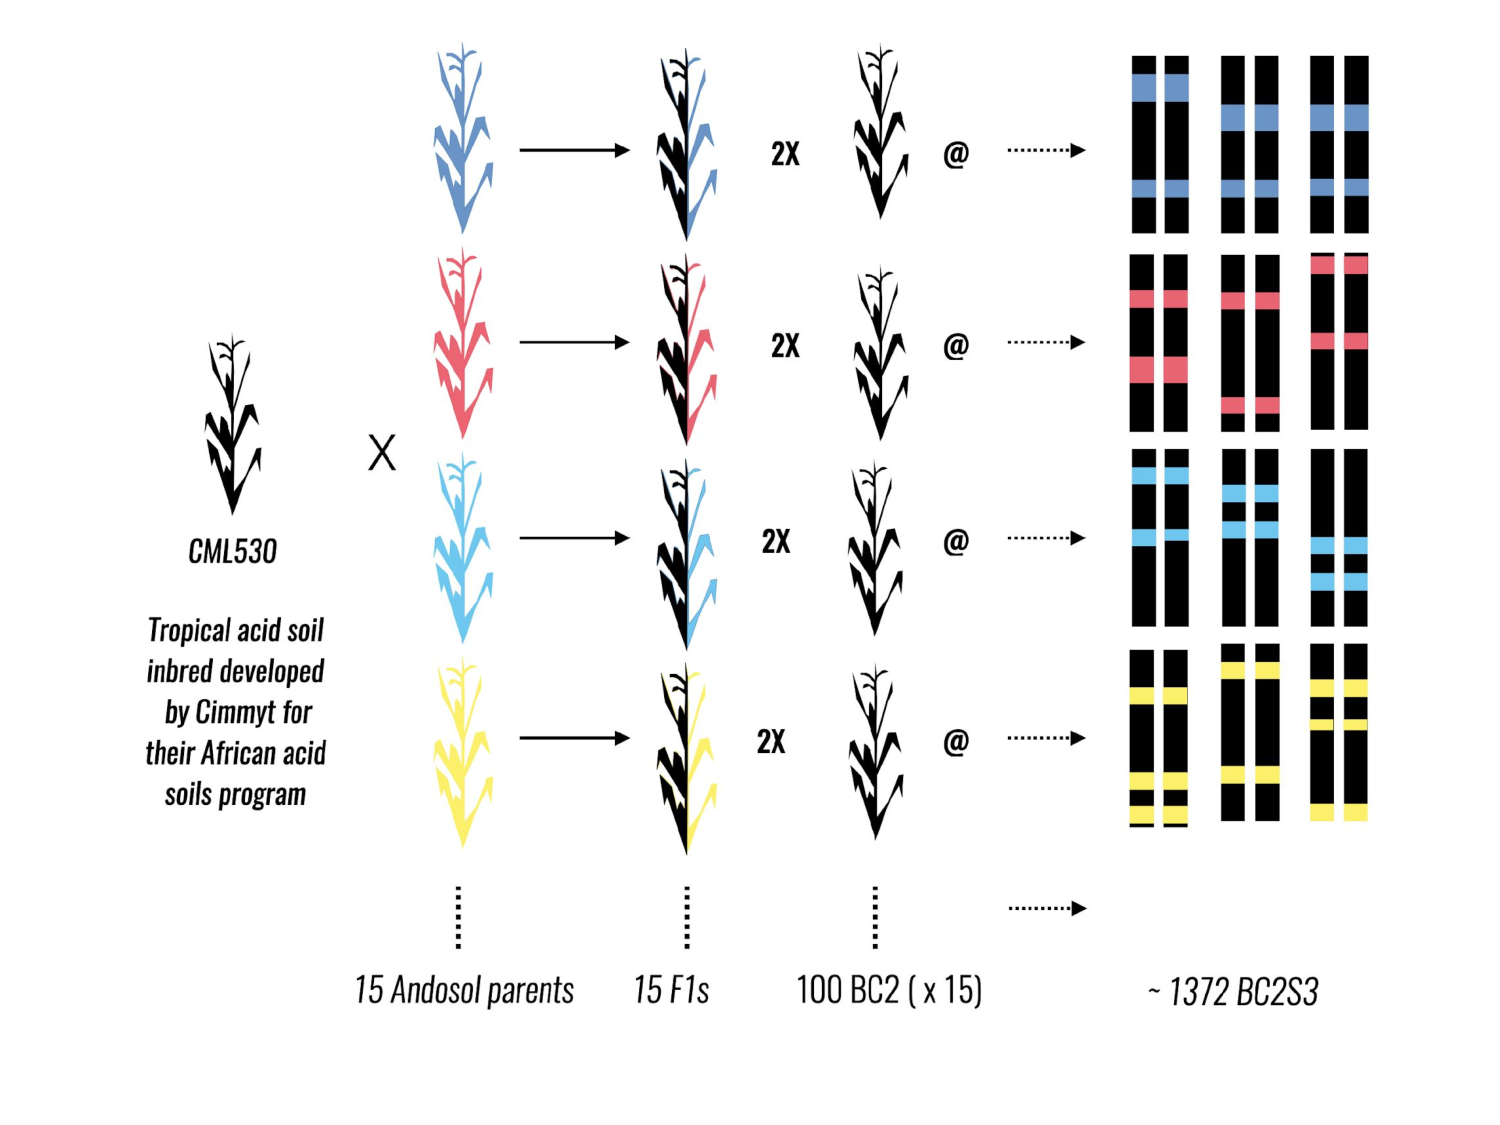
\includegraphics[width=0.8\paperwidth]{Chapter-3/figs/fig-27d.pdf}
\caption{\textbf{Andosol Introgression Resource, AIR, Panel Breeding scheme}
15 landraces were selected from Mexico and Guatemala Andosols to be founders of the populations}
\label{Fig3.0}
\end{figure}
\clearpage

\subsection{Genotyping}
 To genotype the BC$_2$F$_3$ families, we first sequenced the 15 F1 CML530 x landrace founder individuals and the CML530 recurrent parent using Illumina, generating an average of 30x coverage. In total, we generated ~ 85 million SNPs.
 We identified ~101,000 thousand SNPs that were common across all F1 individuals and were heterozygous between the landrace parents and CML530. From this set of SNPs, we used plink's LD Pruning tool to select a subset of SNPs unlikely to be in linkage disequilibrium. Using a window size of 50kb and selecting 5 SNPs per window,  we obtained a final set of ~ 3,000 SNPs.
 We then designed primers for amplicon sequencing using LGC Seq-SNP technology. This technology involves the design of primers flanking SNPs of interest.
 We then designed primers for amplicon sequencing using LGC Seq-SNP technology.
 This technology involves the design of primers flanking SNPs of interest.
 After PCR amplification, samples are sequenced via Illumina. We obtained good amplification of around 2500 markers distributed throughout the genome, sufficient to build and saturate a genetic map using R/QTL \citep{broman2012}

\subsection{ICPMS}.
We selected a representative kernel from each AIR line seed bulk and processed it for ICPMS.
The final concentrations of minerals were calculated as mg of element per kg dry seed weight. We checked for clustering of the ionomics profile regarding andosol donors and mountain range source using a PCA analysis of the mineral content.

\subsection{QTL Mapping}
We used single marker QTL mapping in BC$_2$F$_3$ population according to R/QTL manual \citep{broman2012},  making associations for the 14 traits.  We established the statistical threshold after  1000 permutations of the phenotype with respect to genotypes.  We did both, joint analysis with the whole population data and analysis per donor family.
The joint analysis increases our power to detect signals from similar allelic effects coming from different Andosol donor backgrounds.
And the separate family analysis allows us to detect QTLs unique in each family at the cost of reduced power. To test the quality of and the potential of  our map for mapping phenotypes related to  Andosols, we decided to make  a QTL analysis of two other phenotypes that have presumptive adaptive roles in maize heirlooms to the highlands of Mexico.
We scored both stem macro hairs and  the presence of anthocyanin pigments in stems as binary (presence/absence) traits. 


\section{Results}
\subsection{Ionome diversity}
The minerals quantified by ICPMS have two types of distributions. The most abundant ions (median x-y ppm) including Potassium, Sulfur and Phosphorus, tend to have more symmetrical and approximately normal distributions, while the less abundant ions (median x-y ppm) have a  heavily right-skewed distribution, like boron, nickel and aluminum.
Skewed data might better be log-transformed for linkage mapping purposes, as the associations might be linear with the order of magnitude rather than the untransformed concentration in the kernel. As a matter of fact The first two principal components of a naive PCA on the untransforme data show a separation of contributions according to the type of distribution.
Skewed data minerals,Al, B, Mo, Ni, (Jarque-Bera test FDR <0.05 table, ions sorted by median abundance, with skewdness and kurtosis measurements) have mayor contributions to the second principal component (12.1 \% variance) while the more abundant and symmetrically distributed ions make the bulk of the contributions to the first principal component.
A PCA on log-transformed low abundance minerals might reveal a different variance-covariance structure where the log(abundace) might vary less orthogonally to other minerals. A hierarchical clustering of the minerals on the untransformed space shows again, a tight clustering of the rare long tail distribution minerals, and les well-defined clusters corresponding to mostly bivalent cations and iron, Fe,Mg,Mn,Zn, with P,S,K, with other correlated pairs being Na,K and surprisingly Aluminum and  caclcium . This correlation structure must be reflecting two underlying causes.
First, the similar chemistry and biological functions of the minerals in the plant tissues. And second, their correlated abundance and bioavailability in the soil.
\clearpage
\begin{figure}[!ht]
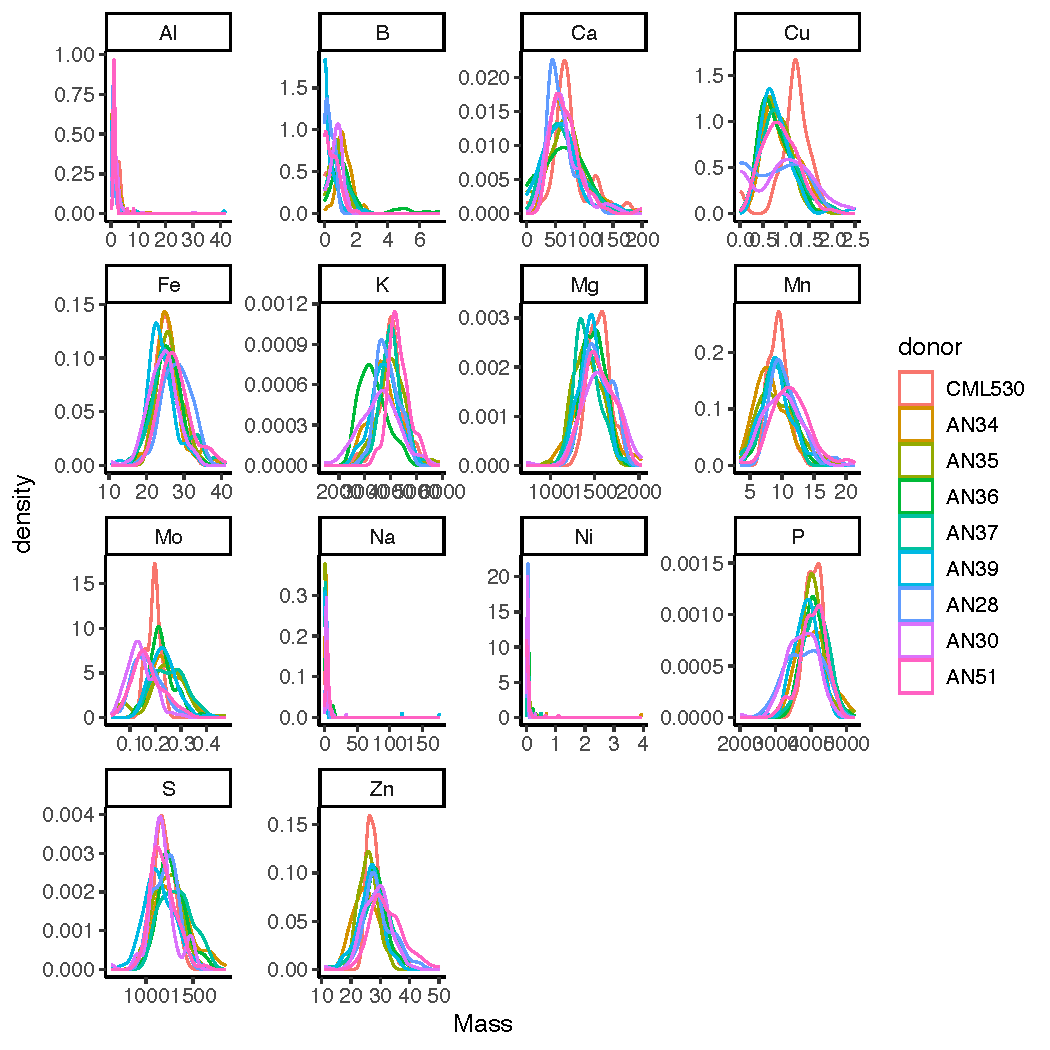
\includegraphics[width=0.8\paperwidth]{Chapter-3/figs/fig3-1.pdf}
\caption{\textbf{Distribution of mineral kernel concentration mg/kg}
Micronutrients have a distribution heavily skewed to the right, linear biological responses might be associated with their log scale (like pH)}
\label{Fig3.1}
\end{figure}
\clearpage

\begin{figure}[!ht]
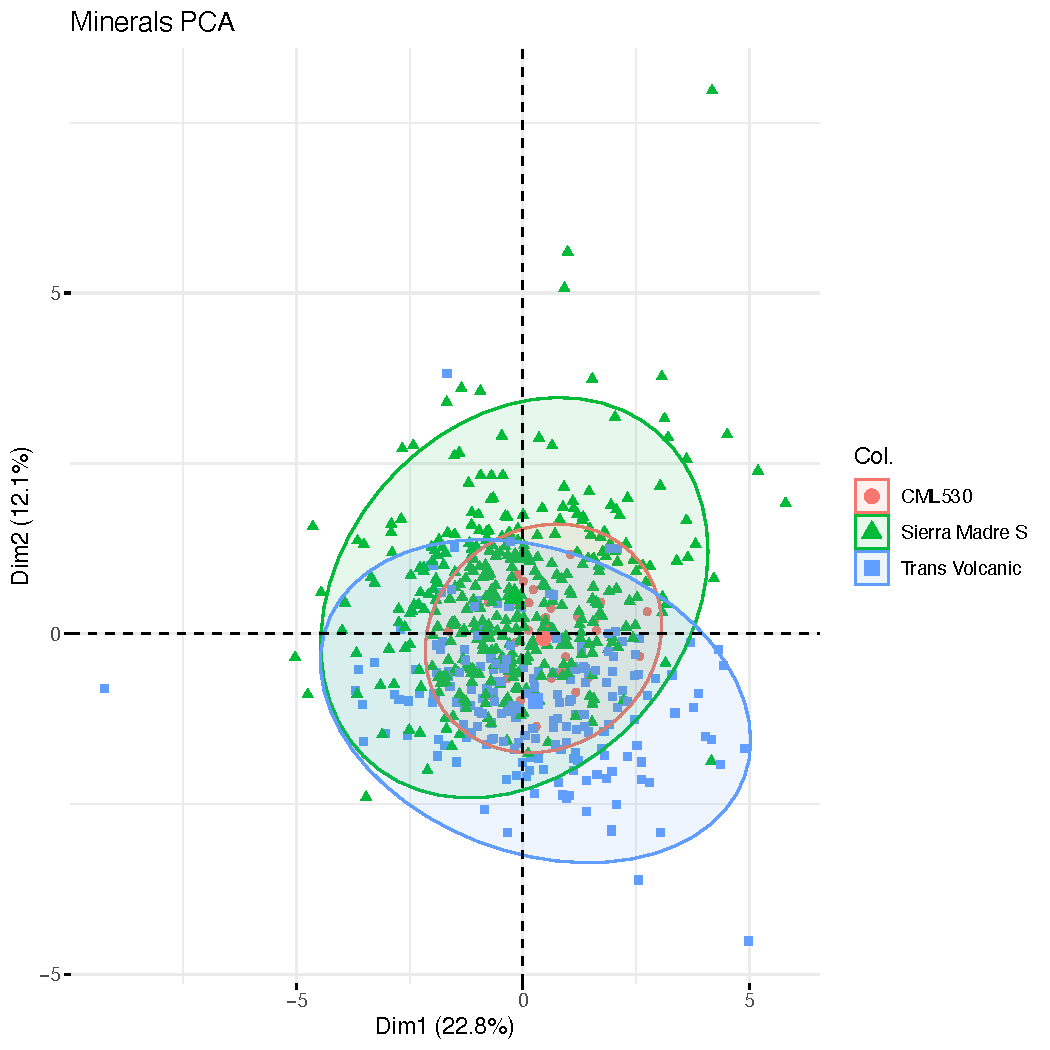
\includegraphics[width=0.8\paperwidth]{Chapter-3/figs/fig3-2.pdf}
\caption{\textbf{Mineral PCA.}First dimension corresponds to variation in macronutrients, second dimension corresponds to variation in less abundant micronutrients}
\label{Fig3.2}
\end{figure}
\clearpage

\subsection{Linkage Map.}
The genetic PCA showed evidence of genetic outliers that most likely are due to contamination.Thus we calculated kinship coefficients (manichakul etal) and discarded x outliers.
We obtained a joint genetic map with 2300 markes of 2500 cM, with mean distance of 1 Mb/cM and sd dev of 1 Mb/cM, no gap grater than 10 cM, in good agreement with our expectations from marker design (mean 1Mb/cM, sd = 1Mb/cM).
Our genotype table has a completenes of 95\%, with mean 95 ccompleteness per marker and 80 ccompletness per individual.
We found a predictable excess of heterozygous given that samples were pooled per row and the genotype calling software penalyzes the homozygote calls.  We found low recombination rates around the reported centromeres (mean sd, t test).
Genetic Maps per individual family varied, as  many alleles were not  polymorphic, and thus excluded, in certain families do to lineage sorting.



\begin{figure}[!ht]
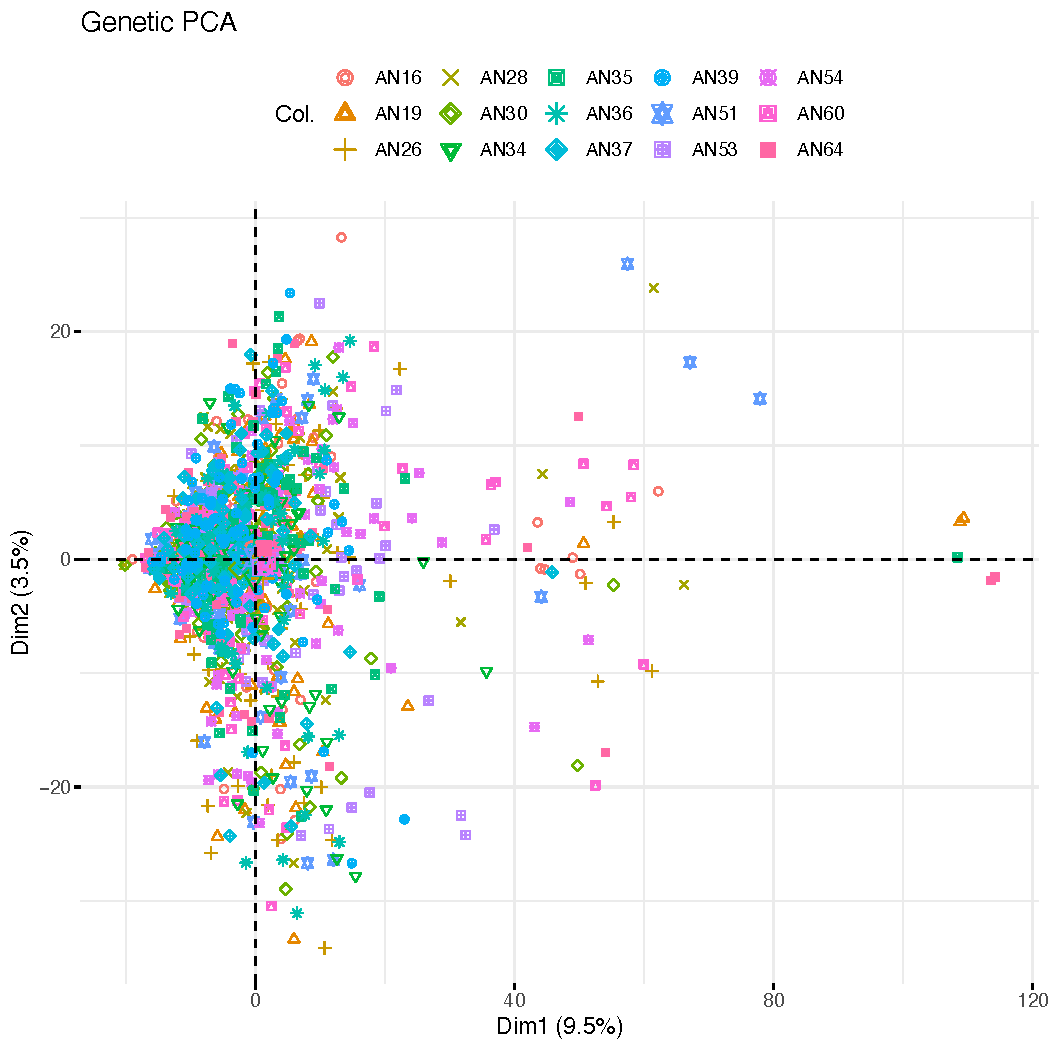
\includegraphics[width=0.8\paperwidth]{Chapter-3/figs/fig3-3.pdf}
\caption{\textbf{Genetic PCA and kinship distribution among AIR lines.}
Dim1 has an enormous contribution to genetic variance, and it is not correlated with either donor or geographical origin. Possible contaminations can be seen in kinship distribution}

\label{Fig3.3}
\end{figure}
\clearpage

\clearpage
\begin{figure}[!ht]
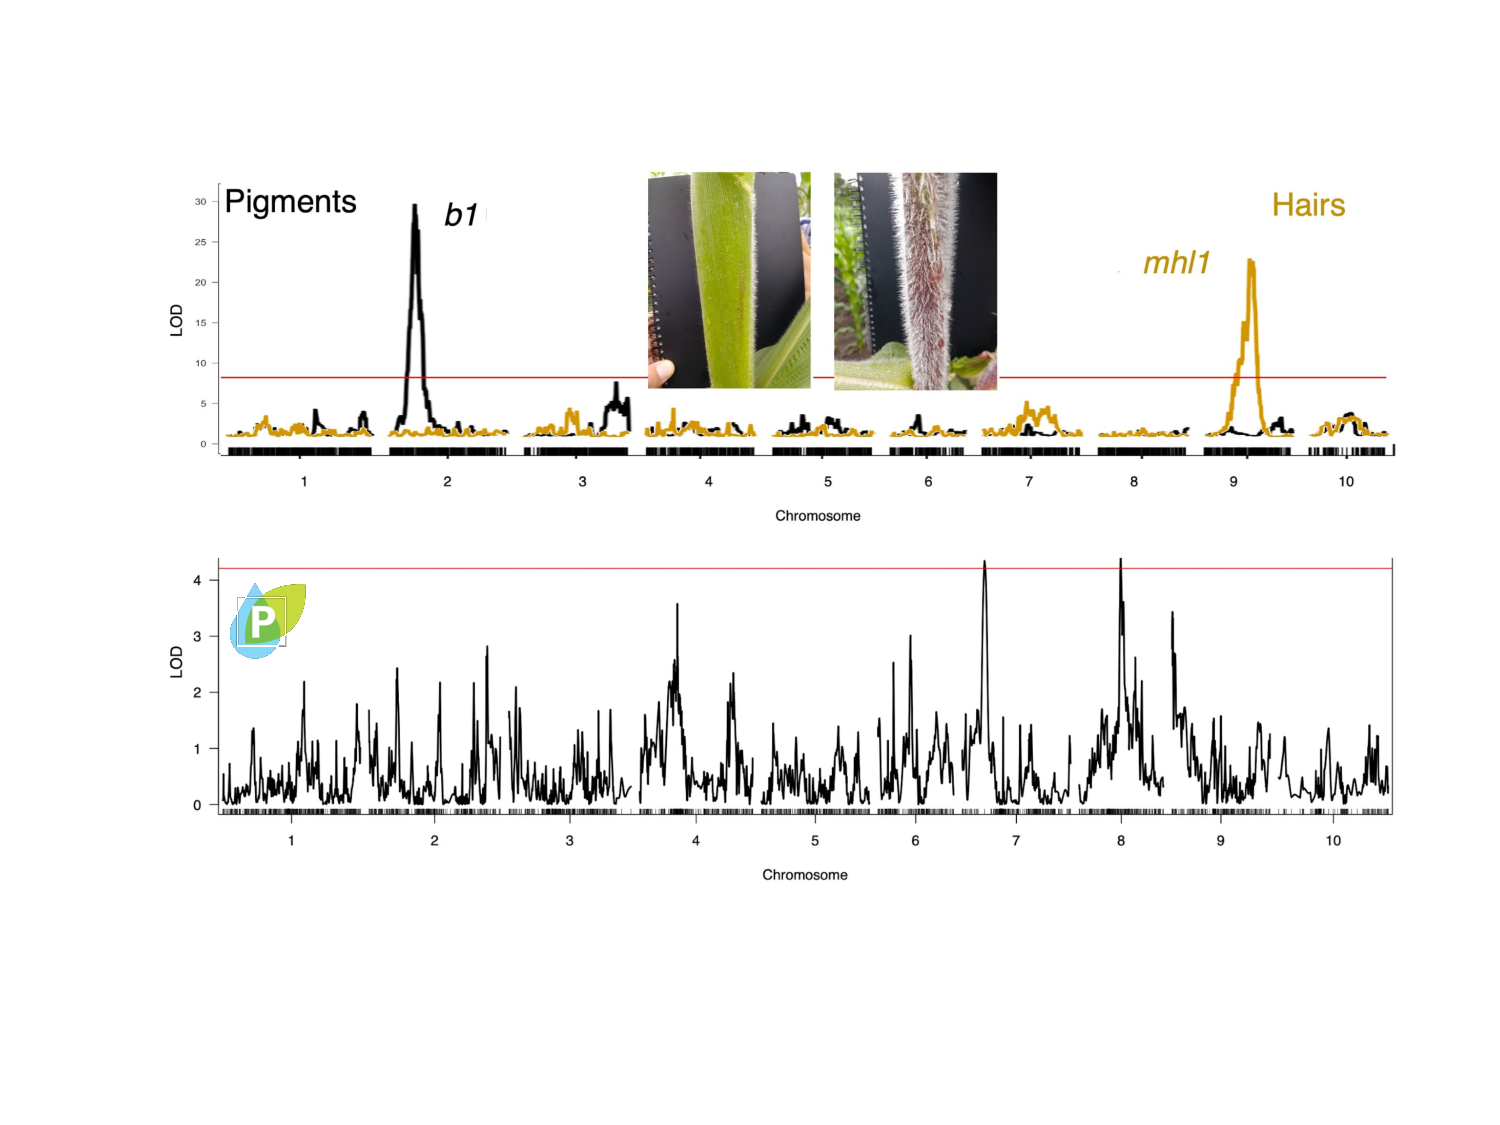
\includegraphics[width=0.8\paperwidth]{Chapter-3/figs/fig-28d.pdf}
\caption{\textbf{QTL Mapping for presumptive Highlandd Adaptive traits and Kernel Phosphorus content} Strong signals were detected for both macro hairs and anthocyanin pigmentation coinciding with previously reported loci \textit{b1} and  \textit{mhl1}.
}
\label{Fig3.1}
\end{figure}
\clearpage

\subsection{QTL Mapping.}
As a quality check we were able to locate strong and highly significant QTLs for stem macro-hairs (LOD =15), and  athocyaning pigments (LOD =20), and colocolaized with previpusly reposrted locis R1 an mhl1.

In the joint map we found genome wide significant single marker QTLs for all minerals measured as described in figure 3. The most significant hits were found for Mn, Mg and Ni.  Of our particular interest Phosphorus showed a robust QTL in chromosome 8.

QTLs that were found in the joint analysis but not in the per family analysis

Family specific QTLs.

QTLs  showing matching  effect sign through families

QTL showing incongroun signs between familes


\begin{figure}[!ht]
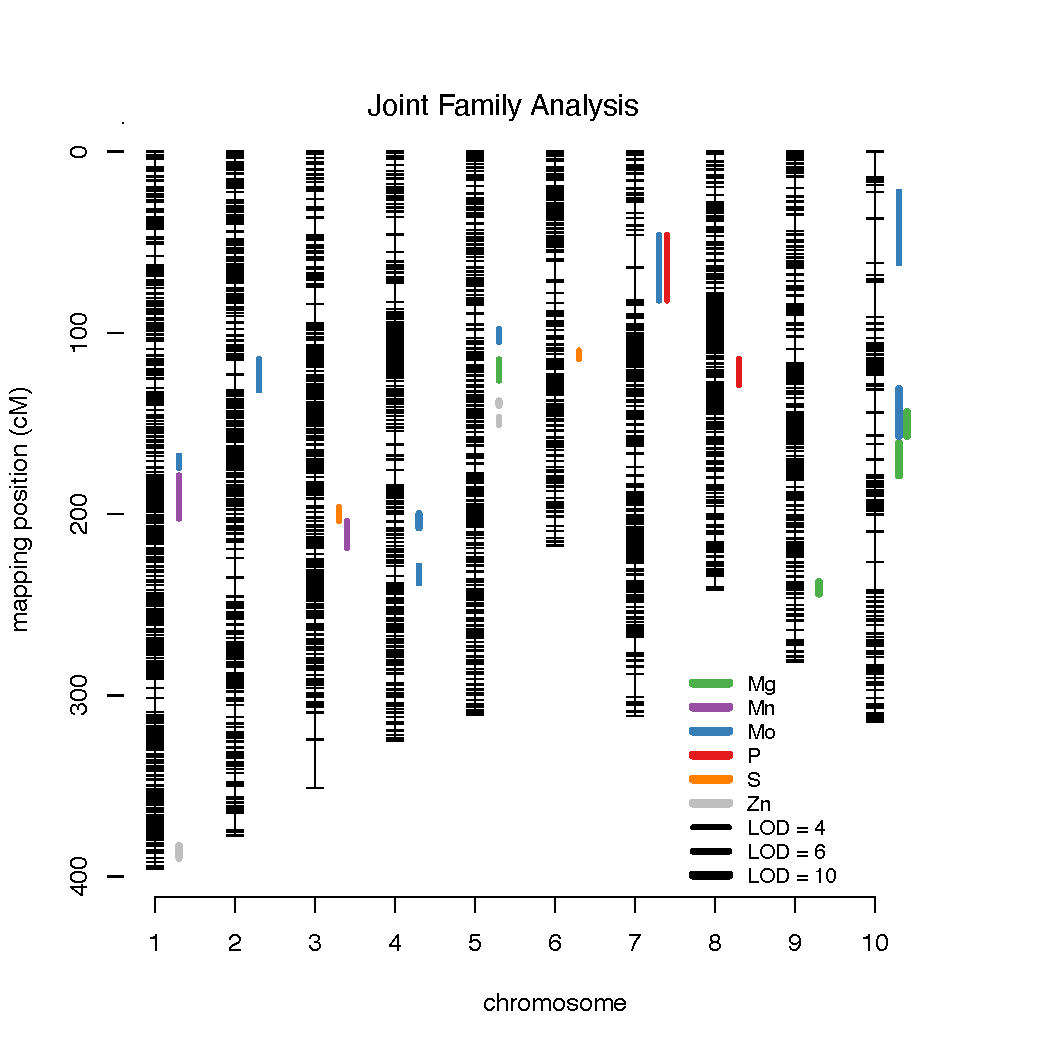
\includegraphics[width=0.8\paperwidth]{Chapter-3/figs/fig3-4.pdf}
\caption{\textbf{Genetic PCA and kinship distribution among AIR lines}
Dim1 has an enormous contribution to genetic variance, and it is not correlated with either donor or geographical origin. Possible contaminations can be seen in kinship distribution}
\label{Fig3.1}
\end{figure}
\clearpage


\subsection{GO analysis of candidate regions}
The total candidate regions (>95\% bayesian confidence intervals) spanned 45 Mb and 567 genes which included 37 gene previously reported as related to mineral nuttrition in plants. There is no overrepresenattion of any biological processes in this span nor in the set of genes closer to the peak qtls. Other peak qtls  markers are located on intergenic regions as expected from theis hiiigherr proportion ( xi squared goodnes of fit). 

\section{Discussion}

\printbibliography[heading=subbibintoc, title=References]

